\documentclass[14pt]{article}

\usepackage{csquotes}
\usepackage{hyperref}
\usepackage{tikz}


\begin{document}


\begin{titlepage}



\newcommand{\HRule}{\rule{\linewidth}{0.5mm}} % Defines a new command for the horizontal lines, change thickness here

\center % Center everything on the page
 
%----------------------------------------------------------------------------------------
%	HEADING SECTIONS
%----------------------------------------------------------------------------------------

%\textsc{\LARGE University Of Helsinki}\\[1.5cm] % Name of your university/college
%\textsc{\Large Research proposal for Doctoral Studies}\\[0.5cm] % Major heading such as course name
%\textsc{\large on}\\[0.5cm] % Minor heading such as course title

%----------------------------------------------------------------------------------------
%	TITLE SECTION
%----------------------------------------------------------------------------------------

\HRule \\[0.4cm]
{ \huge \bfseries Notes}\\[0.4cm] % Title of your document
\HRule \\[1.5cm]
 
%----------------------------------------------------------------------------------------
%	AUTHOR SECTION
%----------------------------------------------------------------------------------------

%----------------------------------------------------------------------------------------
%	DATE SECTION
%----------------------------------------------------------------------------------------

{\large \today}\\[3cm] % Date, change the \today to a set date if you want to be precise

%----------------------------------------------------------------------------------------
%	LOGO SECTION
%----------------------------------------------------------------------------------------

%\includegraphics{Logo}\\[1cm] % Include a department/university logo - this will require the graphicx package
 
%----------------------------------------------------------------------------------------

\vfill % Fill the rest of the page with whitespace

\end{titlepage}

%\newpage

\section*{27th October, 2017}                           

\subsection*{3GPP Document Version Numbering System}
I have studied the system from here: \url{http://www.3gpp.org/specifications/specification-numbering/81-version-numbering-scheme}. I have understood it well.

\subsection*{3GPP Documents Tree}
I have started to study LTE and 5G network from the 3GPP specification documents. I plan to prepare a document tree.

\subsection*{TS 23.401 V 15.1.0}


\section*{3GPP document tree}

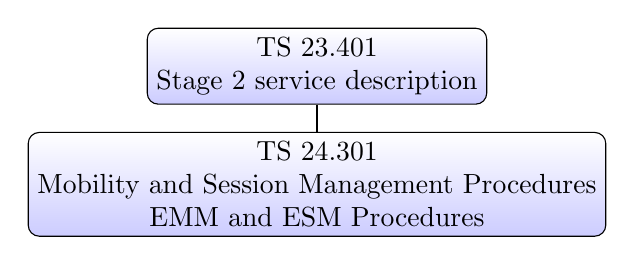
\begin{tikzpicture}[sibling distance=10em,
  every node/.style = {shape=rectangle, rounded corners,
    draw, align=center,
    top color=white, bottom color=blue!20}]]
  \node {TS 23.401\\Stage 2 service description}
    child { node {TS 24.301\\Mobility and Session Management Procedures\\EMM and ESM Procedures} };
\end{tikzpicture}


\section{References}

\end{document}